\documentclass{report}
\usepackage[margin=1in, paperwidth=8.5in, paperheight=11in]{geometry}
%Math packages%
\usepackage{amsmath}
\usepackage{amsthm}
%Spacing%
\usepackage{setspace}
\onehalfspacing
%Lecture number%
\newcommand{\lectureNum}{9}
%Variables - Date and Course%
\newcommand{\curDate}{January 31, 2017}
\newcommand{\course}{CS 240}
%Defining the example tag%
%\theoremstyle{definition}%
\newtheorem{ex}{Example}[section]
%Setting counter given the lecture number%
\setcounter{chapter}{\lectureNum{}}
%Package to insert code%
\usepackage{listings}
\usepackage{courier}
\usepackage{xcolor}
\lstset { 
    tabsize=2,
    breaklines=true,
    language=C++,
    backgroundcolor=\color{blue!8}, % set backgroundcolor
    basicstyle=\footnotesize\ttfamily,% basic font setting
}
%Package to draw trees%
\usepackage{tikz}

\begin{document}
%Note title%
\begin{center}
\begin{Large}
\textsc{\course{} | Lecture \lectureNum{}}
\end{Large}
\end{center} 
\noindent \textit{Bartosz Antczak} \hfill
\textit{Instructor: Eric Schost} \hfill
\textit{\curDate{}}
\rule{\textwidth}{0.4pt}

% Actual Notes%
\section{Dictionaries}
A \textbf{dictionary} is a collection of items, each which contains
\begin{itemize}
\item a \textit{key}
\item some \textit{data} to which the key is mapped to
\end{itemize}
This grouping of keys and data is called a \textit{key-value pair} (KVP). Keys can be compared and are usually unique. Some basic operations we'll use on dictionaries are:
\begin{itemize}
\item \texttt{search(k)}
\item \texttt{insert(k, v)}
\item \texttt{delete(k)}
\end{itemize}
\section{Binary Search Trees (Review)}
A \textbf{binary search tree} (BST) is either empty or contains
\begin{itemize}
\item a KVP
\item a left child BST
\item a right child BST
\end{itemize}
The tree is ordered such that every key in the left child is less than the root key and every key in the right child is greater than the root key.
\subsubsection{BST Search and Insert}
This method takes in one argument \texttt{k} and compares \texttt{k} to the current node (starting at the root), and stops if it's found; otherwise it recurses on both subtrees until it's empty. \texttt{insert(k, v)} uses \texttt{search(k)}, then inserts the key as a new node.
\subsubsection{BST Delete}
This algorithm is slightly harder to implement:
\begin{itemize}
\item If the node we want to delete is a leaf, just delete it
\item If node has one child, move the child up
\item Otherwise, swap with the \textit{successor} or \textit{predecessor} (i.e., the node with the next largest or next smallest key value) node then delete
\end{itemize}
\subsection{Height of a BST}
All of the aforementioned operations on a tree have cost $\Theta(h)$, where $h =$ height of a tree $=$ maximum path length from root to leaf. If $n$ items are inserted one at a time, how big is $h$?
\begin{itemize}
\item Worst-case: $n-1 = \Theta(n)$
\item Best-case: $\lfloor \log(n) \rfloor =\Theta(\log n)$
\item Average-case: $\Theta(\log n)$
\end{itemize}
\section{AVL Trees}
An \textbf{AVL tree} is a BST with an additional constraint:
\begin{center}
\textit{the heights of the left and right subtree differ by at most 1}
\end{center}
At each non-empty node, we store \texttt{height(Right subtree) - height(Left subtree)} $\in \{-1, 0, 1\}$, where
\begin{itemize}
\item -1 means the tree is \textit{left-heavy}
\item 0 means the tree is \textit{balanced}
\item 1 means the tree is \textit{right-heavy}
\end{itemize}
\begin{ex}
A typical AVL (the balance factor is stored in brackets)
\end{ex}
\begin{center}
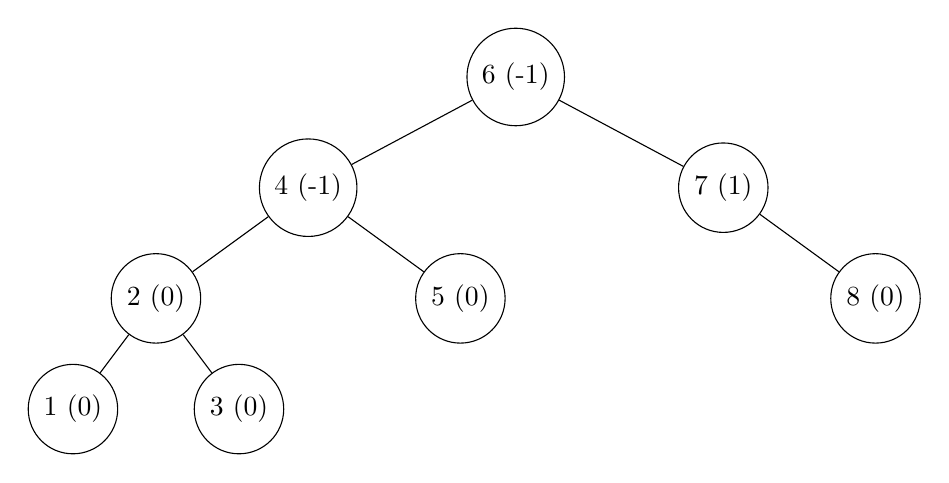
\begin{tikzpicture}[
  level distance=40 pt,
  every node/.style={circle,draw},
  level 1/.style={sibling distance=150 pt},
  level 2/.style={sibling distance=110 pt},
  level 3/.style={sibling distance=60 pt}
]
  \node {6 (-1)}
    child {node {4 (-1)}
    	child { node {2 (0)}
    		child {node {1 (0)}}
    		child {node {3 (0)}}}
    	child { node {5 (0)}}}
    child {node {7 (1)}
      child [missing]
      child {node {8 (0)}}};
\end{tikzpicture}
\end{center}
\subsection{AVL insertion}
To perform \texttt{insert(T, k, v)}:
\begin{itemize}
\item Insert (\texttt{k, v}) in \texttt{T} using usual BST insertion
\item Then from the newly inserted leaf, move up the tree, updating balance factors
\item If the balance factor is $-1$, 0, or 1, then keep going
\item If the balance factor is $\pm 2$, then we call the \texttt{fix} algorithm to rebalance that node (will be outlined later)
\end{itemize}
\subsubsection{Right-rotation}
To fix an unbalanced AVL tree, we want to change the structure of the tree without changing the order (i.e., ensuring that all left children have a smaller key value and all right children have a larger key value). We do this through a special \textit{rotation}:
\begin{figure}[ht]
\begin{center}
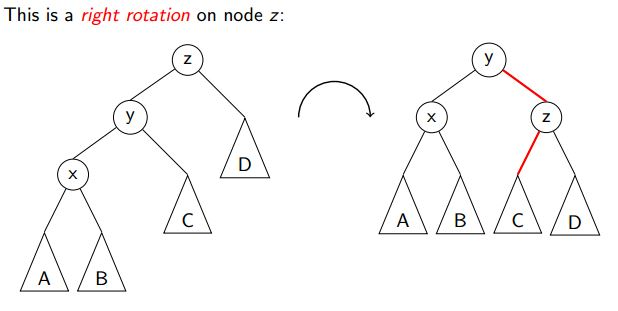
\includegraphics[scale=0.8]{right_rotation.jpg}
\end{center}
\end{figure}\\
The left rotation is the mirror-image of the right rotation. In either case, only two edges need to be moved and two balances updated. The pseudocode for the right rotation is:
\begin{lstlisting}
rotate-right(T)
// T: AVL tree
// This method returns rotated AVL tree
	newroot = T.left
	T.left = newroot.right
	newroot.right = T
	return newroot
\end{lstlisting}
Again, the left-rotation pseudocode is nearly identical. Observe that the runtime of this algorithm is $O(1)$.
\subsubsection{Double Right Rotation}
This function performs two rotations: first, a left rotation on the left subtree. Second, a right rotation on the whole tree:
\begin{figure}[ht]
\begin{center}
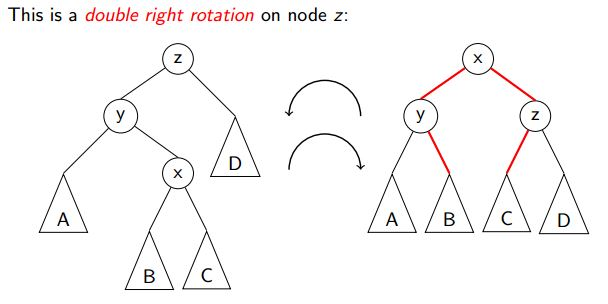
\includegraphics[scale=0.6]{double_right_rotation.jpg}
\end{center}
\end{figure}\\
Similarly, there is also a \textbf{double left rotation}, which is defined as a \textit{right rotation} on the right subtree, followed by a left rotation on the whole tree. The algorithm that will include all of these rotations will be called \texttt{fix}:
\begin{lstlisting}
// T: AVL tree with a balance +- 2
fix(T)
 if (T.balance = -2)
 	if (T.left.balance = 1)
 		T.left = rotate-left(T.left)
 	return rotate-right(T)
 else if (T.balance = 2)
 	if (T.right.balance = -1)
 		T.right = rotate-right(T.right)
 	return rotate-left(T)
\end{lstlisting}
\subsection{AVL Tree Operations}
Just like the BST, we'll use \texttt{search}, \texttt{insert}, and \texttt{delete}:
\begin{itemize}
\item \texttt{search}: same as the BST, costs $\Theta(h)$
\item \texttt{insert}: already dicussed in ``9.3.1: AVL Insertion". Since \texttt{fix} is called at most once, the total cost is $\Theta(h)$
\item \texttt{delete}: first search, then swap with successor (as with BSTs), then move up the tree and apply \texttt{fix}. Here, \texttt{fix} may be called $\Theta(h)$ times
\end{itemize}

%END%
\end{document}